\section{Flip-Flop tipo D con \textit{reset} asíncrono \label{sec:s1}}

\begin{center}
	\begin{minipage}{12cm}
		\begin{tcolorbox}[title=Actividad 1]
			Codificar un flip-flop tipo D con \textit{reset} asíncrono. Compilar y simular. Usar el visor RTL para observar como se implementa el circuito. Configurar en la tarjeta DE2-115, asignar interruptores y un LED.
		\end{tcolorbox}	
	\end{minipage}
\end{center}

La visualización RTL del flip flop tipo D con \textit{reset} asíncrono en Verilog se muestra en la \autoref{fig:ff_d_asyn_rtl}. En el visor se observa que la señal RST se conecta al pin CLRN que sirve para limpiar el estado del flip flop, dicho estado se presenta en el pin SCLR, indicando que al restablecer el circuito, la salida tendrá el valor de esta terminal (cero). Las señales restantes se conectan a los pines correspondientes del modulo (D, CLK y Q).

Las simulaciones para el código en Verilog se visualizan en la \autoref{fig:ff_d_asyn_wave}. Se observa que la salida Q adquiere el valor de la entrada D unicamente cuando en la señal de reloj (CLK) hay un flanco de subida. La limpieza en el flip flop se da de manera asíncrona con el pin RST, ya que no depende de CLK, sino que cuando se tiene un flanco de subida en el \textit{reset}, se ajusta el valor de la salida a 0.

En los Anexos se localiza la descripción del flip flop tipo D con \textit{reset} asíncrono. Se utilizó una lista sensible para el flanco de subida de la señal de reloj y el \textit{reset}. Dentro de esta estructura se empleó la sentencia \textit{if} para comparar el valor de RST: 
\begin{itemize}
	\item Si es 1, se restablece el valor de la salida a 0. 
	\item Si es 0, la salida adquiere el valor de D.
\end{itemize}

\begin{figure}[ht]
	\centering
	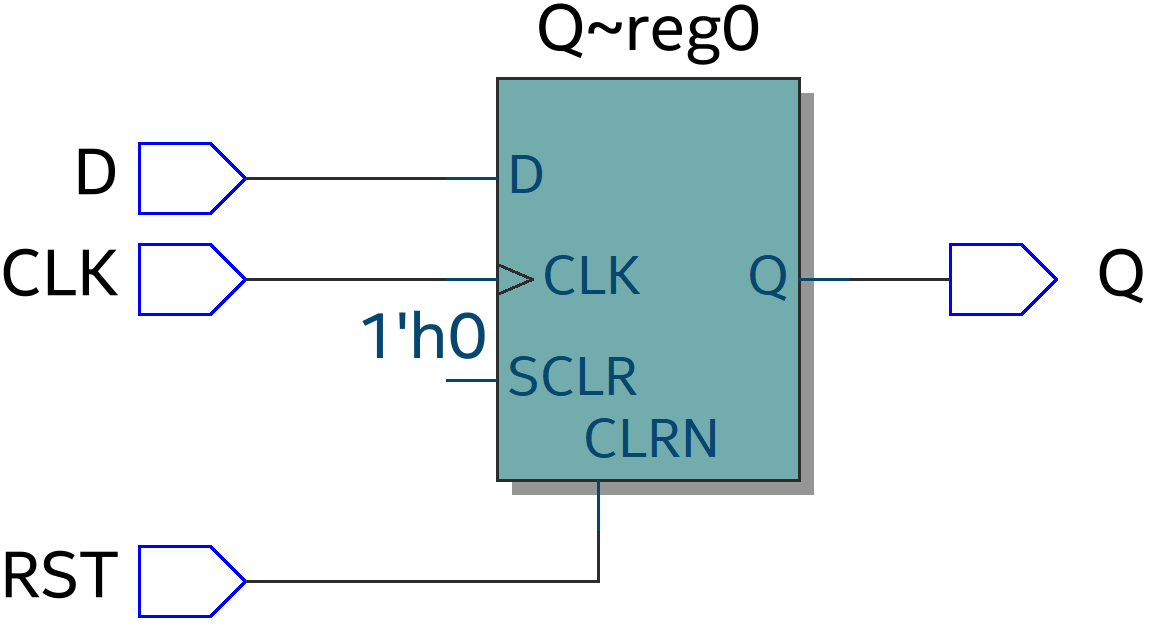
\includegraphics[scale=0.5]{FF_D_Asyn_RST_RTL.png}
	\caption{Diagrama RTL del flip flop tipo D con \textit{reset} asíncrono. \label{fig:ff_d_asyn_rtl}}
\end{figure}

\begin{figure}[ht]
	\centering
	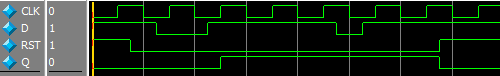
\includegraphics[scale=1.3]{FF_D_Asyn_RST_Wave.png}
	\caption{Simulación del flip flop tipo D con \textit{reset} asíncrono en el visor de formas de onda de ModelSim. \label{fig:ff_d_asyn_wave}}
\end{figure}